% SPDX-License-Identifier: CC-BY-SA-4.0
%
% Copyright (C) 2026 embedded brains GmbH & Co. KG
\documentclass[tikz,border=4pt]{standalone}
\usepackage[T1]{fontenc}
\usepackage[scaled]{helvet}
\renewcommand{\familydefault}{\sfdefault}
\usetikzlibrary{arrows.meta,backgrounds}
\definecolor{ebblue}{HTML}{1F4E79}
\definecolor{boxfill}{HTML}{EAF1F8}
\definecolor{groupfill}{HTML}{F5F5F5}
\definecolor{flow}{HTML}{404040}
\begin{document}
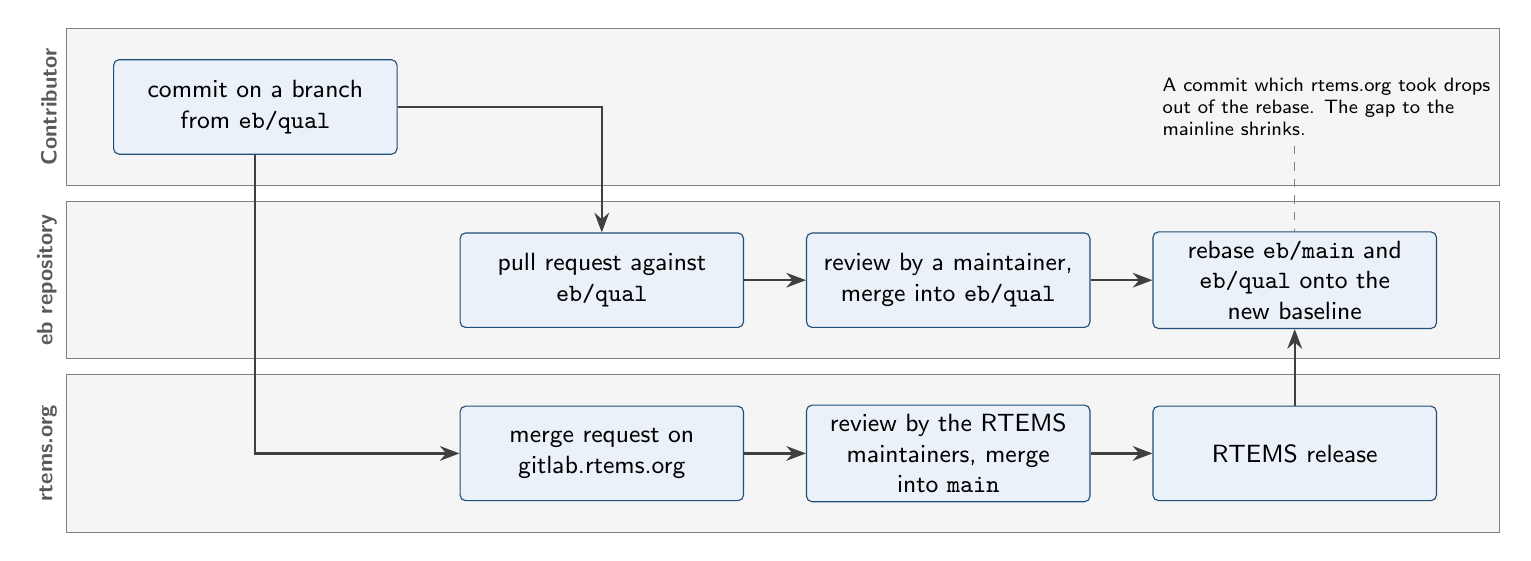
\begin{tikzpicture}[
    font=\small,
    task/.style={draw=ebblue, fill=boxfill, rounded corners=2pt,
      minimum width=36mm, minimum height=12mm, align=center},
    lanelabel/.style={font=\footnotesize\bfseries, text=gray!70!black,
      rotate=90, anchor=south},
    edge/.style={-{Stealth[length=2.5mm]}, thick, draw=flow},
    note/.style={font=\scriptsize, align=flush left, text width=42mm,
      execute at begin node={\hyphenpenalty=10000\relax}}]

  \def\lanewidth{18.2}
  \foreach \y/\name in {2.2/Contributor, 0/eb repository,
      -2.2/rtems.org} {
    \fill[groupfill] (-2.4,\y-1) rectangle (\lanewidth-2.4,\y+1);
    \draw[gray] (-2.4,\y-1) rectangle (\lanewidth-2.4,\y+1);
    \node[lanelabel] at (-2.4,\y) {\name};
  }

  \node[task] (commit) at (0,2.2)
    {commit on a branch\\from \texttt{eb/qual}};
  \node[task] (pr) at (4.4,0)
    {pull request against\\\texttt{eb/qual}};
  \node[task] (mr) at (4.4,-2.2)
    {merge request on\\gitlab.rtems.org};
  \node[task] (merge) at (8.8,0)
    {review by a maintainer,\\merge into \texttt{eb/qual}};
  \node[task] (upstream) at (8.8,-2.2)
    {review by the RTEMS\\maintainers, merge\\into \texttt{main}};
  \node[task] (release) at (13.2,-2.2) {RTEMS release};
  \node[task] (rebase) at (13.2,0)
    {rebase \texttt{eb/main} and\\\texttt{eb/qual} onto the\\new baseline};

  \draw[edge] (commit) -| (pr);
  \draw[edge] (commit) |- (mr);
  \draw[edge] (pr) -- (merge);
  \draw[edge] (mr) -- (upstream);
  \draw[edge] (upstream) -- (release);
  \draw[edge] (merge) -- (rebase);
  \draw[edge] (release) -- (rebase);

  \node[note, anchor=west] (gap) at (11.4,2.2)
    {A commit which rtems.org took drops out of the rebase. The gap to the
     mainline shrinks.};
  \draw[gray, dashed] (gap.south -| rebase) -- (rebase.north);
\end{tikzpicture}
\end{document}
